\chapter{Implementation}

\section{Policy}
The policy is composed of the following parts:

\begin{itemize}
	\item Hardware
	\item Kernel
	\item Binaries
	\item Subjects
	\item Scheduling
\end{itemize}

Each of the main policy parts is presented in the following sections. Preceding
these descriptions is the specification of data types, which are the basis for
the subsequent definition of policy elements.

\subsection{Data types}
This section describes basic data types that are used in the specification of
the system policy. They are referenced in later chapters, illustrating different
parts of the policy.

\input{types.tex}

\subsection{Hardware}
\begin{figure}[h]
	\centering
	\includegraphics[width=\textwidth]{images/xml_hardware.png}
	\caption{Hardware policy}
\end{figure}
\input{hardware.tex}

\subsection{Kernel}
\begin{figure}[h]
	\centering
	\includegraphics[scale=0.6]{images/xml_kernel.png}
	\caption{Kernel policy}
\end{figure}
\input{kernel.tex}

\subsection{Binaries}
\begin{figure}[h]
	\centering
	\includegraphics[scale=0.6]{images/xml_binary.png}
	\caption{Binaries policy}
\end{figure}
\input{binary.tex}

\subsection{Subjects}
\begin{sidewaysfigure}[hp]
	\includegraphics[width=\textwidth]{images/xml_subject.png}
	\caption{Subjects policy}
\end{sidewaysfigure}
\input{subject.tex}

\subsection{Scheduling}
\begin{figure}[h]
	\centering
	\includegraphics[scale=0.6]{images/xml_scheduling.png}
	\caption{Scheduling policy}
\end{figure}
\input{scheduling.tex}

\section{Kernel}
\subsection{Init}
After reset of a x86 system, the processor begins executing code at physical
address \texttt{ffff:0000}, which is mapped to the PC
BIOS\index{BIOS}\footnote{Basic Input/Output System}. The BIOS first performs
tests and initialization routines and then searches for a bootable storage
media. If found, the BIOS copies the first sector of the storage media to
physical address \texttt{0000:7C00} and jumps to this address (i.e. starts
executing code at this address). This is where the system bootloader comes to
live which is responsible to boot operating systems according to its
configuration. Many bootloaders first load additional code from the storage
media and then prepare the environment for OS execution.

The Muen seperation kernel is compliant to the multiboot specification, version
0.6.96 \cite{multiboot}. The multiboot standard is used to uniformly boot
different operating system kernels by multiboot-aware bootloaders.
The Muen kernel exports the required multiboot header within the first 8192
bytes of the OS image. The bootloader loads the OS image into memory according
to the information found in the header and jumps to the physical kernel entry
point specified in this header.

It is the bootloader's task to prepare the system state as demanded by the
multiboot standard, see \cite{multiboot} section 3.2 for details. The system
kernel can except the system to be in this state. After the Muen kernel comes to
live, it performs additional steps before jumping into the main SPARK kernel.
This initial startup code is written in Assembly and conducts the following
tasks:
\begin{enumerate}
	\item Copy the AP trampoline to low-memory, see section
		\ref{subsec:mp-support} \item Initialize per-CPU VMXON regions
	\item Initialize subject VMCS regions
	\item Enable PAE\index{PAE}\footnote{Physical Address Extension}
	\item Initialize per-CPU kernel pagetables
	\item Enable IA-32e mode and execute-disable (NX)
	\item Enable paging, write protection, caching and native FPU error
		reporting
	\item Set up GDT\index{GDT}\footnote{Global Descriptor Table}
	\item Set up Page-Attribute Table (PAT)
	\item Set up kernel stack
	\item Initialize Ada runtime
	\item Jump into kernel main
\end{enumerate}
After this initial steps are executed, the system is in 64-bit IA-32e mode and
all prerequisites are met to enable VMX root operation.

\subsection{Scheduling}
\begin{figure}[h]
	\centering
	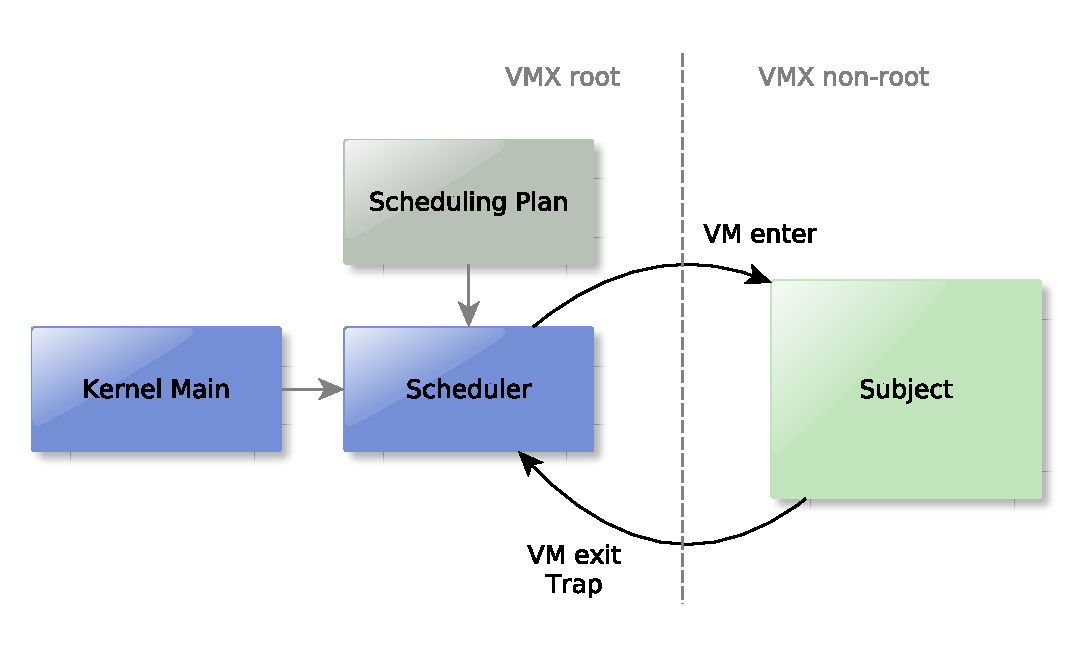
\includegraphics[scale=0.6]{images/scheduler-overview}
	\caption{Kernel scheduler}
	\label{fig:scheduler-overview}
\end{figure}

\subsection{Traps}
\subsection{Exceptions and Interrupts}
\begin{figure}[h]
	\centering
	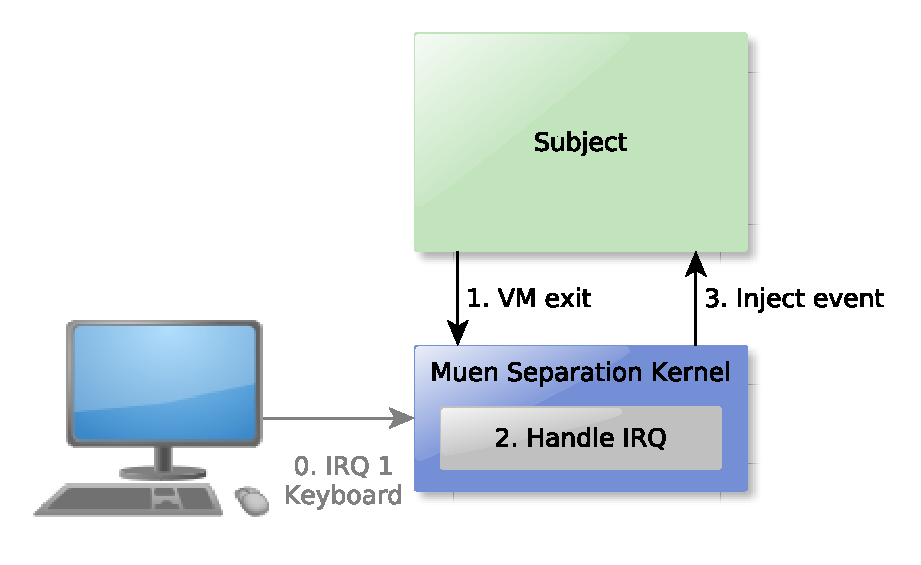
\includegraphics[scale=0.6]{images/external-interrupt}
	\caption{External interrupt handling}
	\label{fig:external-interrupt}
\end{figure}

\subsection{Multicore support}
\begin{figure}[h]
	\centering
	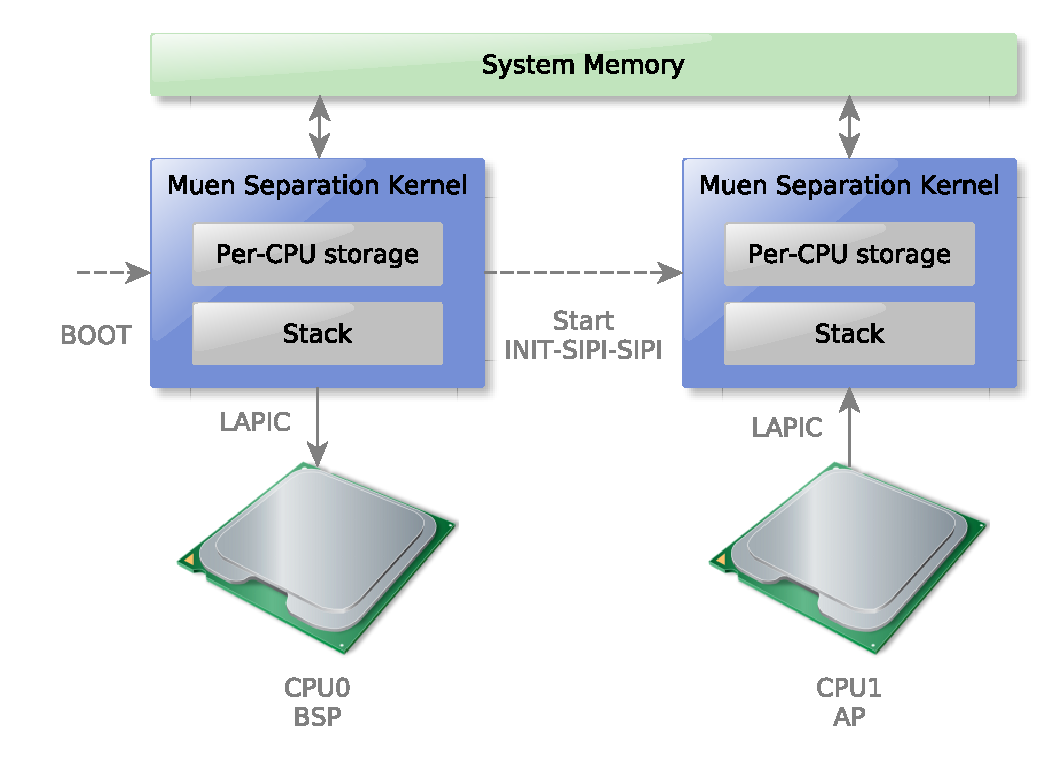
\includegraphics[scale=0.6]{images/mp-overview}
	\caption{Multicore architecture}
	\label{fig:mp-overview}
\end{figure}

\subsection{Events}
\begin{figure}[h]
	\centering
	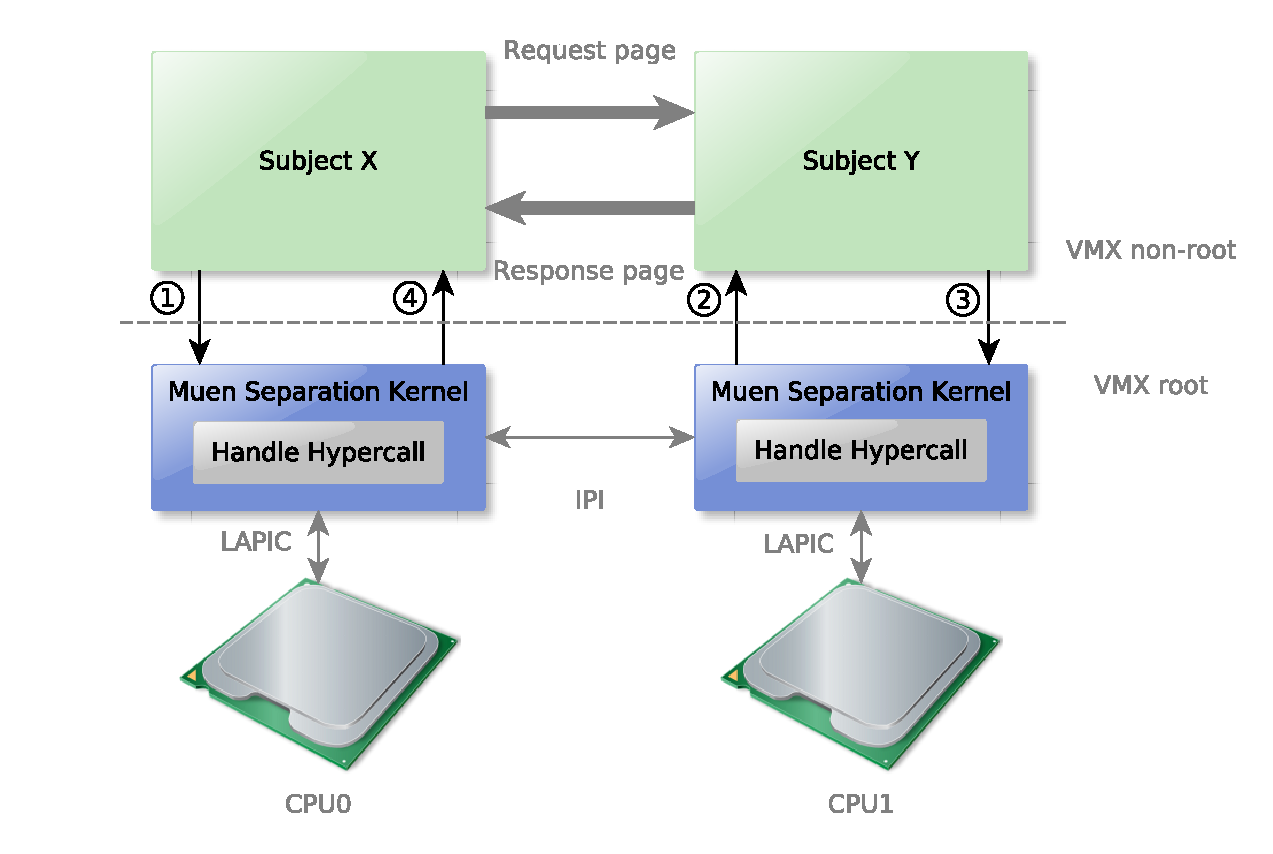
\includegraphics[width=\textwidth]{images/inter-core-events}
	\caption{Inter-core events}
	\label{fig:inter-core-events}
\end{figure}
\section{Build}
\section{Example system}
\begin{figure}[h]
	\centering
	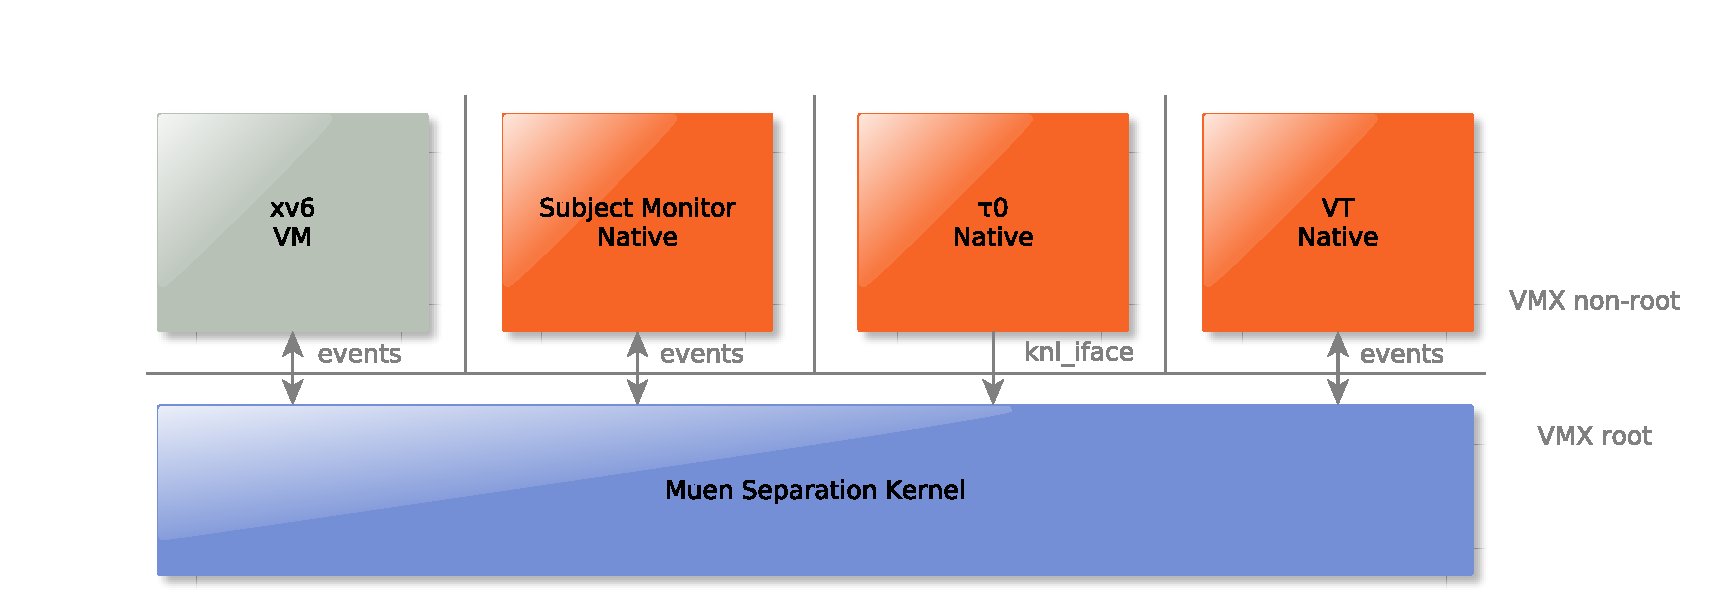
\includegraphics[width=\textwidth]{images/architecture-example_system}
	\caption{Example system}
	\label{fig:example-system}
\end{figure}
